\chapter{Main Work}
\label{chp:quickrollout} 

The main purpose of our study was to create an easy way to utilize the Mesh Potatoes in emergency situations and other situations where there are need for cheap and instant communication. Our main focus has been on providing Internet access to the network, and the aspect of quick roll-out of the network. Internet access may be a vital way of communication in emergency situations, or just convenient in other situations. The process of setting up a mesh network providing Internet should be quick, since time is a crucial factor to consider in emergency situations. In this chapter we will describe parts of the set-up techniques for the Mesh Potatoes. Further on we will present our Emergency Box, which is a box including a Mesh Potato, telephone, solar panel, battery and a charging regulator. A box ready to go in any situations. We will describe how we made this box, and similar work that have been conducted previously on the area. When it comes to the quick roll-out, specific approaches for making a best practice for quick roll-out will be presented. We will present the different types of up-links available to provide the mesh network with Internet access, and give a manual for how connecting the network to the different up-links. In addition to his we will look at the different scenarios of use for the Emergency Box, and how the box best can be utilized in the different scenarios. 

A big part of our work is gathering of information, and make it more understandable for the common user. The existing user guides tend to be advanced and not adapted to the common user, and therefore we found it necessary to make the descriptions easier. The set-up procedures we explain in this chapter can also be found elsewhere. 

*Få litt mer flyt i det avsnittet her

\section{Set-up of the Mesh Potato}
The set-up of the Mesh Potato is a process consisting of, among other activities, installing firmware, allocating IP-addresses and providing Internet to the network. The firmware used for the Mesh Potatoes is called Small Enterprise/Campus Network (SECN) Firmware \cite{ChoosingFirmware}. A flashing process is applied in order to install/update the firmware on the Mesh Potato. See the SECN User Guide for respectively MP01 and MP02 in Appendix \ref{chp:appendixB} and \ref{chp:appendixC} for a more detailed description of how to set up the Mesh Potatoes and how different networks can be built. 


\subsection{Configuring the Mesh Potato}
\label{subsec:configuring}
Configuring a Mesh Potato is the process of allocating an unique IP-address to the MP. Each of the MPs were assigned a static IP address, these addresses were not part of the LAN address space. The IP addresses are allocated in a predefined default address space 10.130.1.20. In order to change this IP address, the MP has to be connected via an Ethernet cable to a PC running Linux. The PC must be on the same subnet as the MP, in order to establish contact. When the PC is on the same subnet, the MPs web interface can be accessed via a browser. In the web interface, the IP of the MP can easily be changed. This description works for both versions of the MP. One difference is that you can change the IP on MP01 by using interactive voice response (IVR) commands (see page 28 in Appendix \ref{chp:appendixB}). A second version of the MP02 is in development. This version has a telephone jack port (FXS daughterboard), which allows for IVR. 

\begin{enumerate}
\item Set the PC to have the same subnet, by writing the following command in the terminal:
\noindent
\begin{lstlisting}[language=bash]
  $ ifconfig eth0 10.130.1.120 netmask 255.255.255.0
\end{lstlisting}
\item Open a browser and type in "10.130.1.20". The web interface will then appear. 
\item In the web interface, under network, change the IP address field to "192.168.1.x", where x is the unique number for the specific MP. This number should be between 21-99. In order to set the change, a save and reboot must be done from the interface. 
\end{enumerate}

\subsection{Upgrading the Mesh Potato}
\label{subsec:upgrading}
The firmware of the Mesh Potatoes are under constant development. It is therefore advisable that the MP is running the latest version of the firmware. The process of upgrading the firmware is different from MP01 and MP02. The different methods are described below. 

\subsubsection{Installing Firmware on Mesh Potato 1.0}
Flashing is the process of updating or changing the firmware (SECN) on the MP01. The most common way to perform the flashing process is by using the potato-flash application \cite{flashing}. This is a specialised software application for the Mesh Potato. Potato-flash can be used regardless of previously installed firmware on the Mesh Potato \cite{InstallingSecnFirmware}. 

\begin{enumerate}
\item Downloaded the 64 bit potato-flash utility from \url{http://download.villagetelco.org/utilities/potato-flash/potato-flash-64bit/} to the folder \textbf{/etc/local/bin}.
\item Made the potato-flash file executable by writing the following command in the Linux terminal.
\begin{lstlisting}[language=bash]
  $ cmod +x /usr/local/bin/potato-flash-x64
\end{lstlisting}
\item Downloaded the rootfs file (\texttt{openwrt-secn1_1-GA01-MP01-root.suashfs}) and the kernel file (\texttt{openwrt-secn1_1-GA01-MP01-vmlinux.lzma})  from \url{http://download.villagetelco.org/firmware/secn/stable/mp/SECN-1.1/} to a folder we called mp\_firmware in our local directory.
\item Opened the terminal and wrote the following commands: 
\end{enumerate}


\begin{framed}
\noindent \textbf{Enter root environment:} 
\begin{lstlisting}[language=bash]
  $ sudo su
\end{lstlisting}

\noindent \textbf{Turn of network manager:}
\begin{lstlisting}[language=bash]
  $ service network-manager stop
\end{lstlisting}

\noindent \textbf{Bring the interface connected to the MP up:}
\begin{lstlisting}[language=bash]
  $ ip link set eth0 up
\end{lstlisting}

\noindent \textbf{Go into the directory containing the .squashfs and .lzma files:}
\begin{lstlisting}[language=bash]
  $ cd <the directory containting the .squashfs and 
  .lzma files>
\end{lstlisting}

\noindent \textbf{Assign IP-address to the interface:}
\begin{lstlisting}[language=bash]
  $ ifconfig eth0 1.1.1.1
\end{lstlisting}

Before running the potato-flash utility we made sure that the MP was unplugged from its power supply, and that the Mesh Potato was connected to our PC via an Ethernet cable. 

\noindent \textbf{Executing the potato-flash utility:}
\begin{lstlisting}[language=bash]
  $ potato-flash-x64 openwrt-secn1_1-GA01-MP01-root.suashfs 
   openwrt-secn1_1-GA01-MP01-vmlinux.lzma
\end{lstlisting}
\end{framed}

Briefly after the potato-flash had been executed, dots stared appearing on the screen, like shown in \fref{fig:flashing}. When these dots started appearing, we plugged the power supply back into the Mesh Potato, and the process of upgrading the firmware started. 

\begin{figure}[t]
  \centering
      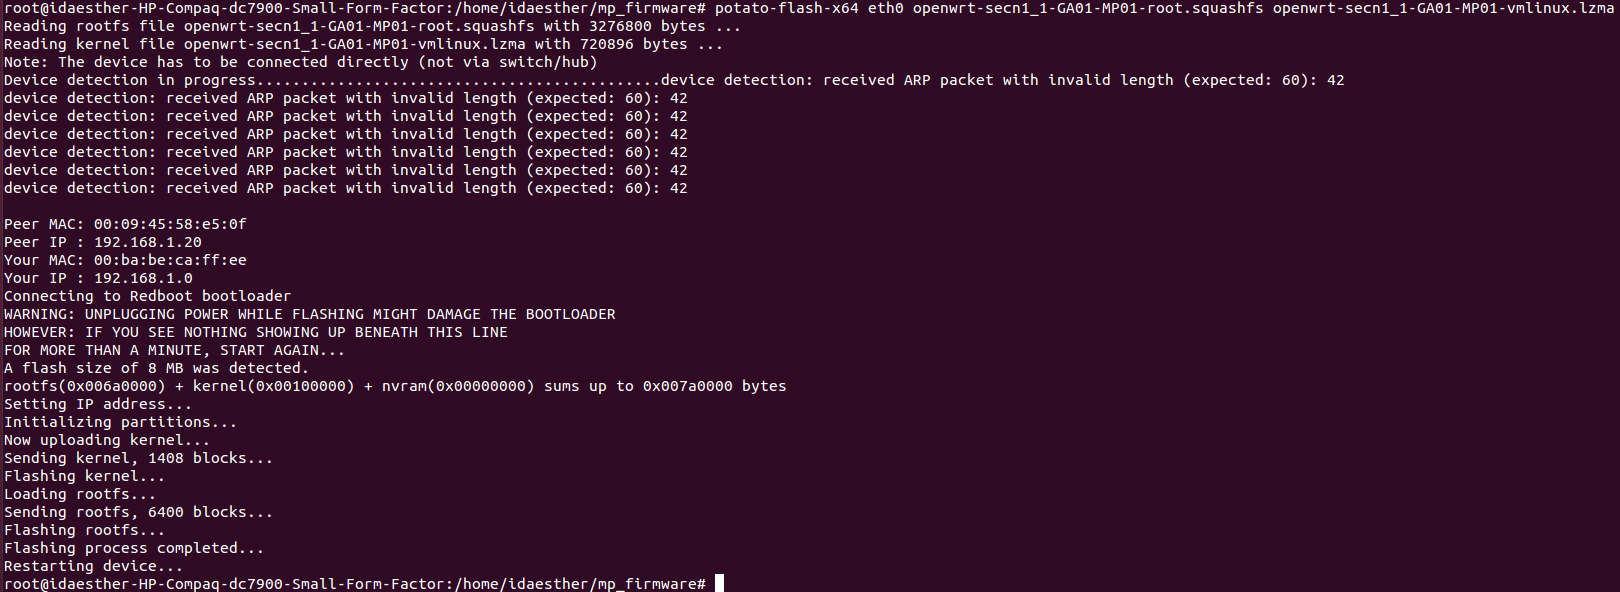
\includegraphics[width=1\textwidth]{potatoFlash.png}
  \caption [Flashing the Mesh Potato]{\textbf{Flashing the Mesh Potato.} This figure shows the flashing process from when we first flashed our Mesh Potato 1.0}
  \label{fig:flashing}
\end{figure}


\subsubsection{Installing Firmware on Mesh Potato v2.0}
The process of upgrading the MP's firmware is simplified with the MP2. With the MP1, command shell must be utilized in order do this. In contrary, with the MP2, firmware upgrade can be done from the SECN web interface (more information about the interface can be found in section \ref{subsec:interface}). Extra functionality has been added to the interface from MP1 to MP2. Under "Advanced" in the interface an extra tab called "Firmware" is added, and there the firmware upgrade can be executed. 

\subsection{The SECN Web Interface for Configuration}
\label{subsec:interface}
Village Telco provides a SECN web interface for configuration and management of individual MPs. This web interface can be accessed by entering the IP address of the MP in a browser, this interface is shown in \fref{fig:webinterface} In order to be able to do this, the PC must be on the same subnet (exact same prefix) as the MP.  

The web interface allows the user to do alterations in the MP. The web interface allows the user to alter some key parameters. Among these are changing the IP address of the device, set up the WiFi Access Point, VoIP/SIP Configurations, Password and Web Server Security. The web interface also allows the user to do changes to more advanced settings and monitoring. To get a detailed description of the web interface see the user guide in Appendix \ref{chp:appendixA}. In addition to this, like mentioned above, the interface has been extended and improved from MP1 to MP2. More actions can be conducted via the interface with MP2. 

\begin{figure}[t]
  \centering
      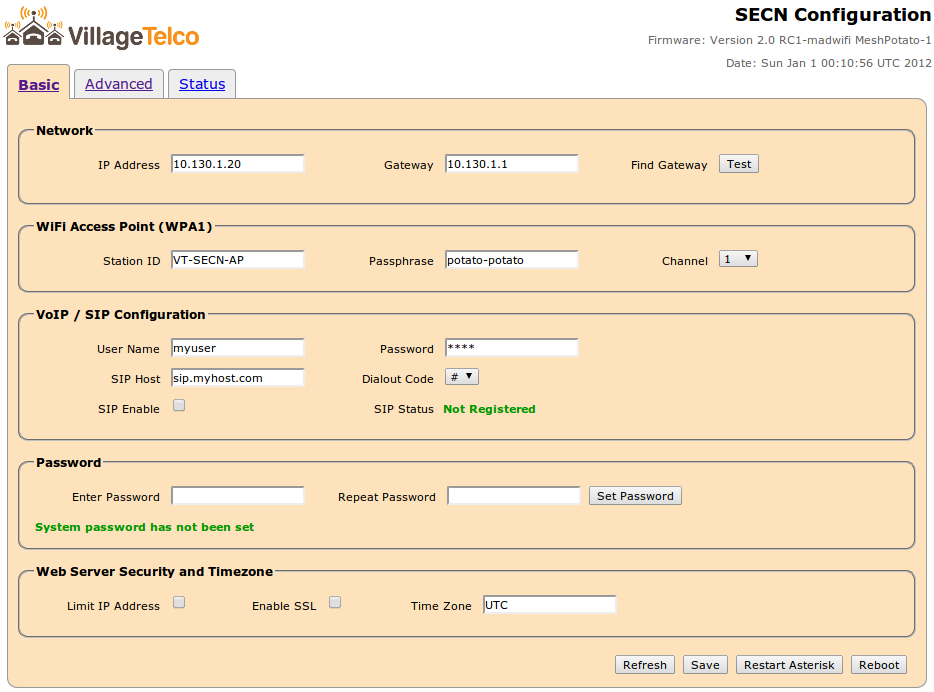
\includegraphics[width=1\textwidth]{webinterface.png}
  \caption [Web interface]{\textbf{Web interface.} Displays the web interface to the Mesh Potato.}
  \label{fig:webinterface}
\end{figure}


\section{The Emergency Box}
The Mesh Potatoes and Village Telcos were created to get voice and data connection to areas where they are non existent or too expensive for the average person. As of now the Mesh Potatoes have been set up to create small or bigger networks in villages all over the world. We want to expand this solution by looking at its mobility and its usage on the go. We want to make a box that has high adaptability, enabling it to easily be used in several different scenarios, under different conditions and by different people all with different needs. The box have to be so easy that there are no room for misunderstanding or mistakes. It should be a to-go box ready for any situations.  
 
\subsection{Previous/similar work}
\paragraph{Go Box.} Something similar has been done before by Keith Williamson, a volunteer in the Village Telco community. His idea of utilizing the Mesh Potatoes in emergency situations started with his interest in amateur radios, and the use of radios in emergency situations. He put together a "go box" by using a waterproof Pelican 1200 case. This case contained a bracket holding the Mesh Potato, a rechargeable Li-Ion or Li-Poly battery, telephone handset and junction box to provide an on/off switch \cite{keith}. Our Emergency Box differ in some ways from the Go Box made by Williamson. 

\paragraph{AfrikaBurn}
AfrikaBurn is a "Burning Man" festival in Tankwa Town in the Karoo (South Africa) that is held once a year \cite{whatisafrikaburn}. This is a festival with focus on art and freedom of expression. Instead of using money, the festival attendants are inspired to trade different types of goods with each other. A Village Telco has been established at this festival a few years now. Free-standing phone boots with Mesh Potatoes powered by solar panels has been set up at the festival area.  \cite{africaburnforavillagetelco,africaburnsagainforavillagetelco}. 

*Skrive mer om utstyret de brukte.


*Hvordan er vår boks annerledes fra Keith sin, hvordan er den satt opp, hvordan er den laget, hvordan fungerer den, forklare ulike komponentene, forklare endringer som gjøres underveis grunnet testing (flere versjoner), ting som gjøres for at den kan rulles ut raskt (feks script). 
%Hvordan er den annerledes fra Keith sin?
%How is the box set up?
%How is it made?
%How does it work?
%Explain the different components
%Explain evt. changes
%Script?

\subsection{Key Components}
The components of our emergency box is described in \tref{tab:components}. 

\begin{center}
\begin{table}[t]
\caption{\label{tab:components}The components of Emergency Box}
    \begin{tabular}{ | l | p{9cm} |}
    \hline
    \textbf{Component} & \textbf{Description and purpose} \\ 
    \hline
    Access point for Internet &  Mesh Potato v2.0\\ 
    \hline
    Suitcase/box &  A suitcase made of high quality plastic coated with aluminium foil. Strengthened edges and corners of aluminium and steel. It has a soft-padded interior, than can be split into different rooms. Two snap locks with keys, and a solid handle for carrying. Dimensions: 455x330x152 (width, depth, height). Weight: 2,6 kg. \\ 
    \hline
    Power supply & A gel battery (12 V and 5 Ah). No need for maintenance. The battery acid is bound in a viscous gel. This prevents leakage, even when the battery is mounted horizontally. Long lifetime and safe to handle. The battery is fully closed, and do not need refill of battery water. No hydrogen gas or other gas might leak. When the battery is charging no gas or acid vapor is emitted, hence the battery can be placed in narrow or enclosed spaces. The battery withstands multiple discharges. The gel battery is ideal for seasonal or occasional use, since it have a slow self-discharge tempo, and a good ability to recover after deep discharging. Dimensions: 114x69x109. Weight: 2,16 kg. \\
    \hline
    Plain old telephone & \\
	\hline
	Solar panel & Solar panel from Multicomp with item number: MC-SP10-GCS. Power rating: 10 W. Power Voltage Max: 17 V. Dimensions: 357x280x18\\
	\hline
	Charging regulator & Regulator for 12 V solar panel. Protects the battery from overcharging and discharge. The charging regulator is connected between the solar panel and the battery to regulate the voltage to the battery. Capacity: 100 W / max. 7 A. Overcharging protection: 14.5 V. Discharge protection: <10,5 V. Three diodes shows charging, high voltage and low battery voltage. \\
	\hline
    \end{tabular}
   \end{table}
\end{center}

\subsection{Creating the Emergency Box}
This section describes how we created the emergency box from scratch. A go-box is delivered with everything already set up. The Mesh Potato is configures and delivered with an unique IP address. In addition the suitcase contains a cd with Linux Ubuntu in case the user does not already have it installed and there would be a need for the user to configure or upgrade the MP. The case would also contain necessary cables and a detailed descriptions on how to connect to the different up-links. 

\paragraph{Conjoining the components of the emergency box.}
The part that binds all the components together is the solar regulator. This is used in order to not overcharge the battery. The solar regulator was initially built for another type of solar panel than the one we chose to use. This, for example, means that the concomitant plugs could not be used. These plugs were cut of and we soldered on our own wires. The solar regulator is connected to all three main components, the solar panel, the battery and the Mesh Potato. 

First we cut of the plugs on the solar regulator and soldered on new wires. Then we cut of part of the MP's power cord and soldered this onto one of the wires. The second wire from the solar regulator was connected to the solar panel. Before doing this we measured how much voltage was in the solar panel and if this voltage was affected by light. This test was done just by holding the solar panel up to a bright lamp. When both the solar panel and the MP's power cord was connected to the regulator, the only thing remaining was the battery. The battery was fully charged and showed a voltage of a little over 13 V. We unplugged the MP and connected the battery. After the battery was attached we powered up the MP, and it worked. 

\paragraph{Configuring and upgrading the emergency box.}
When the emergency box is delivered the Mesh Potato is already set-up and configured with an IP-address, and running the latest version of the firmware. These processes are described in sections \ref{subsec:configuring} and \ref{subsec:upgrading}.


\subsection{Battery and Charging Calculations}
All the calculations done in this section is based on the components described in \tref{tab:components}. 

\paragraph{Charging with solar panel.}
How long it will take for the solar panel to charge the battery from fully discharged to fully charged depends on how much sun there is. The following calculations are calculated using the peak value of the solar panel (10W). 

The solar panel capacity is:
$$Amp = \frac{Watt}{Volt} = \frac{10 W}{17 V} = 0.59 Ampere$$

When charging batteries it is important to take the charging factor into account. This factor is the ratio between supplied capacity and submitted capacity. The charging factor varies depending on type of battery. For our gel battery the factor is roughly 1.2. The charging factor does not have an annotation. 
If the battery is completely discharged it will take: 

$$Amp\times Hours = AmpHours \Rightarrow Hours =\frac{AmpHours}{Amp} = \frac{5 Ah\times 1.2}{0.59 A} = 10.17 Hours$$

to fully charge it. 

This calculation does not take into consideration that the solar panel may have to charge the battery while the MP is running. The effect from the solar panel to the battery will then decrease. 

The capacity from the solar panel will then be: 
$$Amp = \frac{Watt}{Volt} = \frac{10-2.5 W}{17 V} = 0.44 Ampere$$

The time it will take to fully charge the battery from fully discharged condition will then be: 
$$Amp\times Hours = AmpHours \Rightarrow Hours =\frac{AmpHours}{Amp} = \frac{5 Ah\times 1.2}{0.44A} = 13.6 Hours$$

Number of sun hours per day in for example South Africa in December is approximately 14. In June number of sun hours is approximately 10.5. And off course, it can be cloudy, so these numbers are best case. This means that it is possible to fully charge the battery in the course of a day, but it may not always be the case. The following calculations shows how long the battery can provide the Mesh Potato with power from fully charged condition without the solar panel charging it at the same time. 

\paragraph{With Mesh Potato v1.0}
With the components described in \tref{tab:components} the number of hours the MP1 can last with fully charged battery is: 

$$Amp = \frac{Watt}{Volt} = \frac{2.5 W}{12 V} = 0.208 Ampere$$
$$Amp\times Hours = AmpHours \Rightarrow Hours = \frac{AmpHours}{Amp} = \frac{5 Ah}{0.208 A} = 24 Hours$$

\paragraph{With Mesh Potato v2.0}
With the components described in \tref{tab:components} the number of hours the MP2 can last with fully charged battery is: 

$$Amp = \frac{Watt}{Volt} = \frac{? W}{12 V} = ? Ampere$$
$$Amp\times Hours = AmpHours \Rightarrow Hours = \frac{AmpHours}{Amp} = \frac{? Ah}{? A} = ? Hours$$


\subsection{Possible improvements }
As mentioned this set-up is fairly easy and simple, but leaves room for improvements. For a starter there should be an on/off switch to not use unnecessary battery capacity. This on/off switch would be placed between the battery and the regulator. Unless a measuring instrument is available to check the voltage, there is no way to know the remaining battery time. This might be very useful in situations where communication is vital and the hours of battery lifetime should be taken into account.

The battery we used is a gel battery. They are less explosive than the lithium batteries, and are better suited to be placed into enclosed spaces that may get somewhat hot. The downside of the gel batteries is their heavy weight. Since our aim is to make a case that is portable, a lighter battery would be preferable. 

The MP2 is a lot smaller than the first generation, and a powerful solar panel does not take that much space, so there is no need for a suitcase of the size we have purchased. A smaller case that is lighter and easier to handle would make the solution even more portable. 

Our main focus was to get something that worked and that was safe, and we took aesthetics and appearance little into consideration. This is therefore also an area that can be improved. 

* How make it suitable to connect to different up-links, how to the configuration process as easy as possible. 

\section{The Process of Quick Roll-Out}
As mentioned, one of our areas of focus is the process of quick roll-out. There are many aspects that can be included in order to speed up the roll-out process and make it as easy as possible. We will now present some of our ideas to meet this requirement.

\paragraph{Script}
A script is a list of commands that can be executed without user interaction, in other words, to automate a process. In order to connect the mesh network to Internet a list of commands have to be executed. One idea to speed up the process of setting up the network was to create a script to automate this process. One way to do this could be by creating a self-executable script that could be included in the emergency box on for example on an USB-stick. There would have to be a different script, and different USBs, for each up-link type. 

*Forklare spesifikke ting som er tatt i betrakning for å gjøre utrullingen raskest mulig. Feks scripting, manual etc. 

*Hvordan utdele telefonnummer raskt, opplæring av folk. VIKTIG. Hver boks bør ha nummer skrevet på seg allerede, og ferdig satt opp med ip-adresse. 

\subsubsection{With the MP02}
The MP02 Basic does not have the option to connect to a phone. Hence the issue with telephone number distribution is not an issue. Later in 2014 Village Telco will release a new version of the MP2, MP2-Phone. MP2-Phone will be identical to MP2 Basic just with an FXS daughterboard. With this new version the issue of number distribution appears. 

A go-box could be delivered with several MPs, each MP is marked with the preconfigured IP address. Since it is not possible to connect a phone to the MP there is no issue of number distribution. The box could for example contain 5 MPs, where one would be connected to an up-link, while the other ones would be strategically placed in order to spread the internet access further. 

\paragraph{Distributing Numbers}
When a Village Telco is set up today, telephone numbers are distributed by updating a spreadsheet with name and number to the users. These spreadsheets are printed out and delivered to everybody. This is a system that might seem cumbersome, but serves its purpose. If new nodes are added to the network or any changes are made, new sheets have to be printed out and delivered to everybody. This way of spreading telephone numbers might be more difficult with the go-box. 

One option is to continue with the number distribution approach in use today. The suitcase could contain 5 MPs, all MPs are marked with its unique IP address. There will be attached a list with the IP addresses of the other Mesh Potatoes in the suitcase. When setting up the network the names can easily be filled in on each Mesh Potato. Thil will then be the telephone list.  

An other approach would be to integrate the distribution of who belongs to which number in the web interface. A new feature could be implemented in the interface. This feature would discover the other MPs in range, also in range through other MPs. All MPs would be displayed with name of the SSID, IP address, where the last octet is the telephone number and the name of residence ore user. This name could be edited by the master user or by the user themselves. Each MP in the suitcase are preconfigured and set up, they are also set up with security and a password to enter the web interface. So in order for a user to enter the web interface they have to enter the password in order to get access. Once inside they can see other MPs in range and also put in their name, for the other MPs to see. The password and security is set up in so that no other than the main user of the MP, the one having the phone connected, can change the name. 

\section{Up-Link}
Our main focus when deploying the emergency boxes, is to provide Internet to the mesh network. This because it is crucial to have the possibility to communicate with the local community and the outside world during an emergency situation. In 2011, UN declared Internet access a human right \cite{HR}. This says something about the extent of the Internet, and the importance of connectivity. In order to provide Internet to the mesh network formed by the emergency boxes, at least on the Mesh Potatoes must be connected to an access network via an uplink. An uplink connects a device or a LAN to a larger network \cite{uplink}. Which type of access network that is available depends of the location. Some places there might exist a stable landline, other places not. Then an option could be to use satellite or cellular networks. It is therefore important that the emergency box has high adaptability in order to fit different scenarios. The availability of the different uplinks is not the only thing that vary. The up-link speed and the price also varies from place to place, and between the types of uplinks. In the following sections, we will look at some of the uplinks available, and how Internet access can be provided to the mesh network.  

\subsection{Internet via Telephone-line}
The most common way of getting Internet access is via a landline. The telephone lines are most often used for this, since they can be converted to broadband. In this way it can be used for phone calls and Internet simultaneously \cite{internet}. The line is usually in the form of twisted pairs (copper lines). These lines support broadband up to 10 Mbps, and are often in form of ADSL, or other digital subscriber line of type x (xDSL) technologies \citep{audestad}. Internet via telephone lines can be provided as a stand-alone solution, or it can be provided together with television or/and phone service. The latter option is usually cheaper. Internet through landlines have a high reliability \cite{cablevssatellite} in comparison to satellite and cellular network. We will now shorty describe some technologies for getting Internet access via a telephone line; dial-up Internet connection, ISDN, and DSL. Although dial-up Internet connection is practically extinct in developed countries, we will include it here due to the different application scenarios for the emergency box. 

\subsubsection{Dial-up Internet connection}
Dial-up is an analogue technology that utilizes the telephone line. A telephone wall jack is used as a fixed point of connection, and the computer is connected to a voiceband modem. With this technology, the data is transmitted over the same frequencies used for phone calls. Hence, if you only have one telephone line, you cannot take a phone call and use Internet at the same time \cite{differentuplinks}. The absolute maximum speed is 56 kbps. Along with the digital era, better internet technologies were introduced; ISDN and DSL. 

\subsubsection{ISDN}
Integrated Services Digital Network (ISDN) is a fixed internet connection, which also utilizes the telephone lines. When using ISDN, as with dial-up, a telephone wall jack is used as a fixed point of connection. But ISDN utilizes a ISDN terminal adapter instead of voiceband modem. This ISDN terminal adapter sends out digital signals. The data speed varies between 64 kbps - 129 kbps. The speed of the data is symmetric, which means upstream and downstream data rates are the same. In contrary to dial-up, ISDN allows voice calls and transmission of data simultaneously. ISDN is faster than dial-up, but the speed is nothing compared to the speed obtained using DSL \cite{differentuplinks}. 

\subsubsection{DSL}
Digital subscriber line (DSL) is, like the name indicates, a digital high-speed technology for Internet access that allows simultaneous voice and data transfer. Like dial-up and ISDN, DSL also run over the telephone lines. With DSL the data is not converted between analogue and digital signals. Despite this, the signals are modulated in order to be transferred on non-voice frequencies. DSL is an always-on technology, and in this way differ from the previous technologies mentioned. Only a small part of the telephone line is used for voice signals. The DSL technology allows utilization of a unused frequency spectrum of a telephone line, hence making it possible to transmit data faster. When the voice and data signals arrive at the telephone company's local switching station, they are separated and routed differently; voice to regular telephone system and data to the ISP, and then the Internet. A connection must be within approximately 5 kilometres of a station in order for DSL to work. The speed depends on many factors. Data can be transported up to 6 Mbps (distance of approximately 2 kilometres). Relevant factors that have an impact on the speed is distance to the switching station, and the quality of the telephone line. Like mentioned earlier, there are different types of DSLs. The most common is ADSL, where the A stands for asymmetric; the downstream speed is faster than the upstream speed \cite{differentuplinks}.

\subsubsection{Quickly Connect a MP01 to the Internet via Ethernet Cable}

These instructions requires that the MP01 is new or factory reset, so that no former configurations will affect the following set-up. 

\begin{enumerate}
\item Make sure that the Mesh Potato is connected to a PC running Linux with an Ethernet cable. 
\item The default IP address of the MPs are 10.130.1.20, so in order to access the MP, the PC must be on the same subnet. To do this write in the terminal: 
\noindent
\begin{lstlisting}[language=bash]
  $ ifconfig eth0 up 10.130.1.120 netmask 255.255.255.0
\end{lstlisting}
\item Enter the SECN web interface by typing the IP address (10.130.1.20) of the MP01 in a browser. 
\item Change the IP address under "Network" to 192.168.1.x (Where x is a number between 21 and 99. If it is the first MP that is set-up it is normal to choose 21). Press "Save and Reboot" in the interface. Wait for the MP to reboot. 
\item Open Linux terminal and type in the following command: 
\noindent
\begin{lstlisting}[language=bash]
  $ sudo su
  $ ifconfig eth0 172.31.255.253 netmask 255.255.255.252 
\end{lstlisting}
\item Telnet into the MP01:
\noindent
\begin{lstlisting}[language=bash]
  $ telnet 172.31.255.254 
\end{lstlisting}
You have now entered the root environment of the MP01. 
\item Execute udhcpc: 
*Skrive hva denne kommandoen gjør
\noindent
\begin{lstlisting}[language=bash]
  $ udhcpc -i eth0 
\end{lstlisting}
You will get a message stating that the udhcpc process has started. This is followed by several messages stating "Sending discover...". When this appears unplug the Ethernet cable connected to the PC, and connect it with an Ethernet cable to cabled Internet (wall). 
*Finne ut hva internett i veggen heter på engelsk.
\item Internet will now be available for the mesh network. The SSID and password for the network can be found and altered in the interface. 
\end{enumerate}



If you have a PC supporting wireless Internet, there are different ways of getting wireless Internet to it. You can get WiFi on your PC from a router with landline connection, or the PC can establish a wireless connection to a access point for example in form of a cell phone. The cell phone may have a cellular network available. On most new smart phones, you can set your phone to act as an access point (AP), so that other devices can connect to it and get Internet. You can off course connect directly to this AP, but then the MP does not get Internet, and can not spread it further on to several neighbour MPs. The following set-up works for both types; either if you connect to a regular wireless router that gets Internet from for instance xDSL or if you connect to a AP that have a cellular network (3G, 4G) available. 

In order to perform this set up, a PC with Linux Ubuntu with wireless Internet, and a Mesh Potato 2.0 is required. The last octet of the IP address of the MP, is the unique number for each MP. The Mesh Potato is pre-configured with an unique IP address which is stated on the MP. In the following example we use "x" as the last octet. When conducting this description please change the x with the last octet written on your MP.

\begin{enumerate}
\item Connect the MP to the PC, running Linux Ubuntu, with an Ethernet cable. The Ethernet cable must be put into the LAN-port on the MP. 

\item Open Linux terminal and install telnet, dns and iptables by entering the following commands: 
\noindent
\begin{lstlisting}[language=bash]
 $ sudo su
 $ apt-get install telnetd
 $ /etc/init.d/openbsd-inetd restart 
 $ apt-get install dnsmasq
\end{lstlisting}

\item The Mesh Potato will be pre-configured and the IP address 192.168.1.x. In in order to access the MP, the PC must be on the same subnet. To do this write in the terminal: 
\noindent
\begin{lstlisting}[language=bash]
  $ ifconfig eth0 up 192.168.1.2
\end{lstlisting}

\item Open a browser on your PC and type in "192.168.1.x" in the URL field. The SECN Web Interface should now appear. This assures you that you have contact with the Mesh Potato. Changes in the interface will be described further down, so do not close this window.  

\item Go back to the terminal and write the following commands in order to set up the ip tables correctly. You might have to change the "eth0" and "eth1", depending on how your laptop is set up. The eth0 in the following commands is equivalent to the interface of the Ethernet port connected to the MP, while the eth1 is the interface to the wireless network. 
\noindent
\begin{lstlisting}[language=bash]
  $ iptables --table nat --append POSTROUTING --out-interface
   eth1 -j MASQUERADE
  $ iptables --append FORWARD --in-interface eth0 -j ACCEPT
  $ echo 1 > /proc/sys/net/ipv4/ip_forward
\end{lstlisting} 
\begin{itemize}
\item If you mess up in this step, accidentally write something wrong etc., the following commands will reset the ip tables, and you may try step 5 again.
\noindent
\begin{lstlisting}[language=bash]
  $ iptables --table nat --flush
  $ iptables --flush
  $ iptables --delete-chain
\end{lstlisting}
\end{itemize}  

\item Telnet into the \gls{mp} and configure the default gateway by entering the following commands
\begin{lstlisting}[language=bash]
  $ telnet 192.168.1.x
  $ route 
  $ route del default 
  $ route add default gateway 192.168.1.2
\end{lstlisting} 

\item Go back to the web interface and click on the "Advanced"-tab at the top of the page. Change the following parameters under "DHCP Server":
\begin{itemize}
\item Tick the box "Enable DHCP Server".
\item Remove the tick from "Use device IP".
\item Change the address in "Gateway Router" to "192.168.1.2".
\item Press "Save" at the bottom of the page. 
\end{itemize}

\item Internet should now be available in the mesh network. A device can connect to the network with the SSID (name of network) stated on the emergency box. This SSID is also stated in the web interface under "WiFi Access Point".  
\end{enumerate}


In order to connect the Mesh Potato network to Internet via a land-line, at least one MP have to be in reach for a Internet signal. Preferably The MP should be connected with an Ethernet cable, but could also be done wireless.  First the Mesh Potatoes have to be configured following the steps below. After completing the steps one can plug the Ethernet cable in in one MP and the internet is spread to the the other MPs in reach. It could be smart to change the name and the password for the different MPs. This is easily done by opening the web interface for each MP. 

When connection to a wireless access point the configuration differs a little bit.

\subsection{Cellular Network Technologies}

\begin{figure}[b]
  \centering
      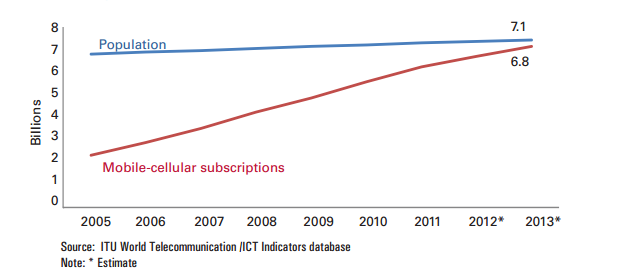
\includegraphics[width=1\textwidth]{mobilesubscriptions.png}
  \caption [Number of mobile-cellular subscriptions]{\textbf{Number of mobile-cellular subscriptions} The figure shows that the growth of mobile-cellular subscriptions have increased drastically during the last decade, and show that there are almost as many as there are people in the world \cite{itu2013}.}
  \label{fig:subscribers}
\end{figure}

%ITU2011-artikkel
It is getting more and more common to use cellular technologies for broadband. Around 2011 the number of mobile-broadband subscriptions grew to twice as many as the number of fixed-broadband subscriptions. In developed countries it is common to have a fixed-broadband connection, and use a mobile-broadband network in addition to the fixed. In developing countries on the other hand, it is not a given that there is access to a fixed-broadband connection. Then mobile-broadband can be the only method of access available. In 2011, 90 \% of the world's population had 2G coverage, and 45 \% had 3G coverage \cite{itu2011}. By 2013, the number of mobile-cellular subscriptions had reached a high level, and were approaching the number of people in the world, like shown in \fref{fig:subscribers}. From 2011 to 2013, the number of mobile-broadband  subscriptions more than doubled in developing countries \cite{itu2013}. 

Through mobile network technologies, high-speed Internet access can be provided via portable devices. In order to get mobile broadband, there must be a cellular network (GSM, CDMA) service available. The key technologies when talking about mobile broadband is 3G and 4G (respectively third and fourth generation wireless networks) \cite{mobilebroadband}. With 3G the average speed is 0.5 to 1.5 Mbps, and with 4G the average speed is 2 to 12 Mbps. These vary, due to different versions of each technology, underlying service etc. Like with everything else, the actual and realistic speed differ from the peak speed \cite{3gvs4g}. 

\subsubsection{Quickly Connect the Emergency Box to Cellular Network}
*Forklare hvordan man raskest mulig kobler nødboksen til akkurat denne type uplink.
%3G via TP-links til mesh nettverket?


\subsection{Satellite}
%ulovlig i feks india, hva skjer da? http://en.wikipedia.org/wiki/Satellite_phone
Internet from satellites are offered by a satellite Internet provider \cite{cablevssatellite}. The satellite are orbiting the Earth, and get signals from a land based Internet connection. To get Internet broadband via satellite you need a satellite dish. The main advantage of using satellite is that it provides an universally available Internet access \cite{broadband}. Since it is universally available, it is fitted for use in rural regions where there exists no landlines or other options for connecting to the Internet. There also exists disadvantages with using satellite-Internet. Since it is a shared medium, privacy concerns arise, and the speed are dependent of simultaneous use. Also the connection can be affected by bad weather, unlike for a wired connection, hence it is not as reliable as cable. 

\subsubsection{Quickly Connect the Emergency Box to Satellite}
*Forklare hvordan man raskest mulig kobler nødboksen til akkurat denne type uplink.
*Normalt er det ethernet ut på disse satelittmodemene

\subsection{Summary Up-Links}

\begin{center}
\begin{table}[!h]
\caption{\label{tab:uplinks}Advantages and disadvantages - Up-links \cite{comparisonuplinks}.}
    \begin{tabular}{ | l | p{4cm} | p{5cm} |}
    \hline
    \textbf{Up-links} & \textbf{Advantages} & \textbf{Disadvantages} \\ 
    \hline
    Landline/xDSL & High reliability, cost effective, good speed. & Low availability in rural areas. \\ 
    \hline
     Cellular networks & High availability, fitted for "on the move"-use. & Expensive, slower than xDSL.\\
    \hline
    Satellite & High availability.  & Unreliable, expensive, slower than landline.\\ 
    \hline
    \end{tabular}
   \end{table}
\end{center}

*Forklare ulikhetene og likhetene ved å koble nødboksen til de forskjellige uplinkene. 

\section{Future Internet Access Methods}
Different methods of distributing Internet is always under development. The previous up-links described is well established, but in many parts of the world not fully developed or not affordable to the average person. The large technology companies, like Google, are experimenting with different ways of distributing Internet. 

\subsection{Google's Internet Balloons}
The majority of the world today is not connected to the Internet. Two thirds of the worlds population does not have access. Project Loon, a Google project, is a network of high altitude balloons travelling in the stratosphere, and through this network be able to give Internet to the Entire world. Cost effective, reliable and inexpensive internet connection to everybody. The project started in June 2013 as a experiment in New Zealand \cite{loon}. 

\begin{figure}
        \centering
        \begin{subfigure}[t]{0.43\textwidth}
                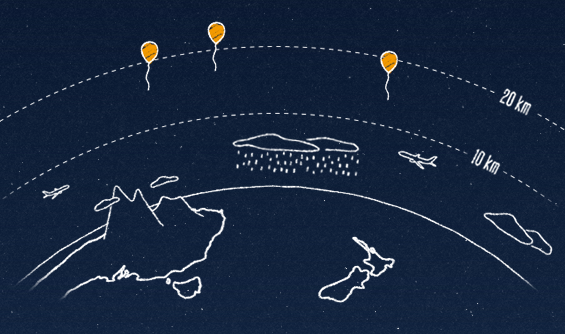
\includegraphics[width=\textwidth]{loon2.PNG}
                \caption[The Balloons are situated in the stratosphere]{\textbf{The Balloons are situated in the stratosphere.}} 
                \label{fig:loonStratosphere}
        \end{subfigure}%
        ~ %add desired spacing between images, e. g. ~, \quad, \qquad etc.
          %(or a blank line to force the subfigure onto a new line)
        \begin{subfigure}[t]{0.415\textwidth}
                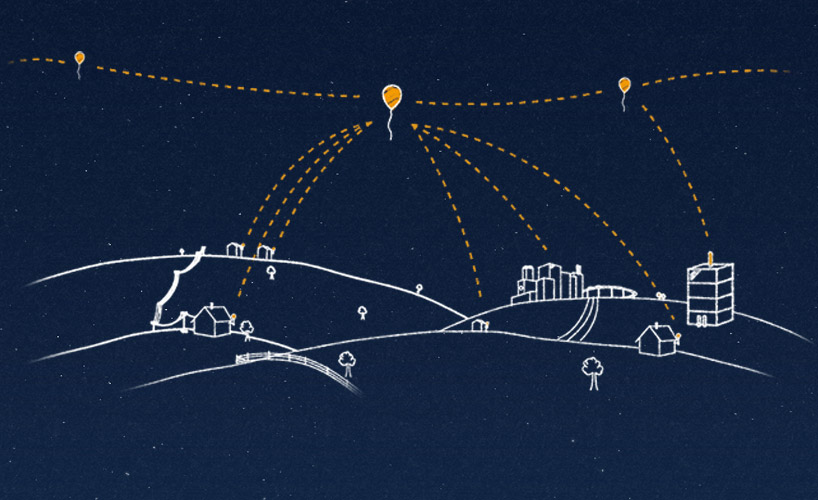
\includegraphics[width=\textwidth]{loon1.jpg}
               \caption[Connecting to the Internet]							{\textbf{Connecting to the Internet}} 
                \label{fig:loonConnect}
        \end{subfigure}
        ~ %add desired spacing between images, e. g. ~, \quad, \qquad etc.
          %(or a blank line to force the subfigure onto a new line)
        \caption{Project Loon: Balloon-powered internet for everyone.}\label{fig:loon}
\end{figure}

The balloons are 15 meter in diameter. They travel about 20 km up in the air, in the stratosphere, twice as high as airplanes and weather, this is shown in \fref{fig:loonStratosphere}. At this altitude there are many layers of wind, each varies in direction and speed. By regulating which wind the balloons are flying in it is possible to control their position, and steer them in the desired direction. \fref{fig:loonConnect} show that  people can connect to the Internet shared by the balloons by having a special antenna attached to their house. From this antenna the signal bounces to one balloon which again bounces through the other balloons and down to the Local Internet Provider on earth. This creates a network in the sky. 

In order to control the altitude of the balloon, it is a specially designed control system. The system is managed remotely from the ground. By either pumping air in, or letting air out of the balloon, one can decide in what layer of air the balloon should be in. Letting air in and out is not the only way to decide whether the balloon should go up or down, but it is the only way to do so in huge scale. A GPS is attached to each balloon in order to keep track of precise positions and see how the winds are changing. There are enormous amounts of data collected, and some of this information is given to meteorologists. The balloons are flying at the same speed as the wind.  

The balloons contains specially designed antennas and radio systems. This in order to receive signals from Project Loon only, and to achieve high bandwidth over long distances. Satellites stay at the same place and at the same altitude. This means that the satellite dish can be mounted in the right direction. This is not the case with the balloons, they are in constant movement and they also vary in attitude. A fixed pointing dish would therefore not work. The antenna needs more sensitivity to an angle than it does straight up, which results in a uniform signal strength. 

Since the balloons are in constant movement, it is important to make sure that there always is a balloon available and one ready to move in when one move out so that the connectivity always are available. If not this project would not be of much use. Every balloon contains information about all the other balloons in order to spread out nicely. Think of it as a flock of birds, they always look at the one next to them and space out perfectly.

The balloons are solely run on solar power. The balloon works as a communication tower in the sky. The solar panels catches the sunlight that is available during the day, as well as charging up the lithium-ion battery to last the night. In the stratosphere it is -70 degrees Celsius, these extreme cold conditions are not ideal fro the lithium battery. In order to make sure that the battery does not loose its effective battery capacity it is important that the battery is kept warm. The battery pack is insulated to reflect the heat that comes of the electronics to stay warm. This is still under development. 

When it comes to lifetime, the goal is that the balloons stay alive for 100 days, or 3 laps around the globe. It is important to make sure that the balloon is leak free. The material is under a lot of stress, air is constantly being pumped in and out to control the position. As well as the extreme cold and warm temperatures. 

Both on the way up and down the air traffic control in the specific country have to be contacted since the balloons go through airspace. Project loon requested permission to land on Norwegian soil according to Teknisk Ukeblad, a Norwegian science magazine. This permission was approved \cite{loonTU}.

The area of usage is enormous. Situations where the Internet infrastructure has not been built out, either because it is too expensive or just not possible. Emergency situations, natural disaster and other situations where the cellphone-towers are down. Project Loon is still a project in development with extensive testing taking place. The project are taking into use what everybody have in common, namely the sky, to reach out to all the areas where access has not been possible. It is expensive to have enough balloons in the sky in order to have good enough coverage. Also the speed is not really high. And even though a specialized antenna is required to get access, this is breakthrough in order to get the whole world connected \cite{loonYouTube, loonNorsk}.

Although this solution is not an option for distributing Internet as of today, it could be a good option in the near future. The solution is affordable and well compatible with our emergency box solution.

Iridium satellite consultation is a large group of satellites providing data and and voice services to specialized satellite phones. The consultation exists of 66 active satellites in orbit. Iridium are considered to be low-orbit satellites and are situated at a hight of 781 km. The Iridium network is unique in the fact that it covers the whole earth, including oceans, airways and poles. The low orbit satellite differs from the balloons in the way that the satellites travel almost 40 times higher above earth and that they stay in a fixed position over the earth \cite{iridium}. To be able to utilize the satellite one would need a specialized satellite phone or a satellite dish in order to receive signal. With the balloons there are only need for an antenna to receive the signal. But then again the balloons does not offer a voice service. The balloons are intended as a cheaper, easier and simpler solution to the satellites.                                         

\section{Apple's Mesh Network}
In March 2014 a new iOS app was released, FireChat. FireChat utilizes Apple's Multipeer Connectivity Framework introduced in iOS7 \cite{appleMesh}. This app enables the possibility to chat with people "off-the-grid" \cite{fireChat}. Applications that communicates through this framework creates a mesh network similar to the one created by the Mesh Potatoes. 

The Multipeer Connectivity framework provides support for discovering services provided by nearby iOS devices using peer-to-peer Wi-Fi, infrastructure Wi-Fi networks and bluetooth to communicate with those services. This communication could either be message-based data, streaming data and resources such as files \cite{multipeer}. These technologies have a short range, but this range can be greatly extended by a chain of users that creates a mesh network, see section \ref{subsec:mesh} for more information about mesh networks. AirDrop is a product that have been on the market for a while and also utilizes mesh networks. The main difference is that FireChat is fully decentralized and peer-to-peer. When there are multiple users in one area FireChat relay messages in the same way as Internet, from node to node, just in this case it is from phone to phone.  This, not only, enables two users to chat with each other without Internet connection, but also far beyond Wi-Fi and Bluetooth range from each other, using the chain of users (phones). For example if Bob is connected to Alice, and Alice is connected to Carol, Bob and Carol can send messages to each other. This chain can be indefinitely long. As long as no one device goes out of Wi-Fi range, all the devices can communicate with each other. 

This new framework will mainstream wireless mesh networking. This could open for a future way of spreading Internet access. This could for example be a hotel basement, cave or rural areas where there are no cellphone towers, or disaster situations where Wi-Fi or mobile broadband  is no longer available. There are many benefits with the use of mesh networks. Mesh networks does not require a centralized infrastructure, there are no need for all the devices to be connected to Internet (as a router). Another benefit is that the mesh network is really easy to set up - everybody just uses the app FireChat (or similar applications like AirDrop), the network is created and everybody is connected. Simple as that! 

The possibilities for this feature are enormous. Both in the creation of applications but also the area of usage. In a lot of countries Internet and mobile broadband connection is extremely expensive, people might afford a used cellphone but not the cost to connect. With this new feature, Internet connectivity can be spread through the mesh network needing only one node (phone) to have internet access. This way of spreading connectivity can open the possibility for people in rural, poorer areas like slums and small villages to stay connected. But not only the poor and rural areas can benefit from this new mesh-networking feature. Young people that does not have a phone can use an iPad or similar to talk to their friends. Or teens with restricted cell contracts can still connect with their friends, just with the help of the neighbours kids phone. Since FireChat enables communication without the use of internet it can be a useful tool to communicate privately and also to send sensitive data.
 
It is not only Apple that is seizing the enormous potential in main-streaming mesh networking. Google has also expressed that they are working on a home mesh network \cite{googleMesh}. FireChat and AirDrop is just the beginning. We believe more extensive and mind blowing applications are to come. 
 
\section{Different Scenarios Where a Quick Roll-out is Necessary}
%What are the specific need for the different scenarios? What adjustments are necessary?

Everyday there are situations all over the world that in some way affects the modern communications systems, or causes a need for one.  These situations can range from big natural disasters, like the tsunami in Japan, to temporary refugee camps and IDP camps. Also more festive situations can have use of the quick roll-out system, for example music festivals. 

\subsection{Natural Disasters}
%Asia og Sør-Amerika
%Philippines - contact Kenneth Bjerkelund to find out their needs for internet etc. makingchange.no. 
A Natural disaster is defined as; \textit{any event or force of nature that has catastrophic consequences, such as avalanche, earthquake, flood, forest fire, hurricane, lightning, tornado, tsunami, and volcanic eruption} \cite{naturalDisaster}.

All over the world relief organizations are ready to help if an unexpected situation occur. These groups of people have the equipment, knowledge, experience and funding to help people in desperate need. Where are they needed? Or if they hear about the disaster and the first respond team are on place, how do they report back about the situation? How do they communicate with each other to work more effectively and help the ones in desperate need? There is no doubt that there is a need for a simple, fast, and reliable communication system.

When a natural disaster hits it is hard to know the extent of it, which  again makes it difficult to predict how the communication systems would be affected. This unpredictability makes it important to always have a backup plan to the backup plan. 
%kanskje flere eksempler her?

History shows that cellphone service is not a reliable service during an emergency situation. During 9/11 the system became heavily overloaded, and when hurricane Katrina hit, 70\% of the cell phone towers where knocked down. One might think that if they live in a big metropolitan that they would be safer, but this is not necessarily the case \cite{disasterComm}. These are situations in the western world. 

When looking at the less developed world, which is often more vulnerable to natural disasters, the situations are different. According to \cite{DevelopingWorld, 360} developing countries are in an larger extent affected by natural disasters than the developed world. The reason for this can be explained by the economic status of the country. Both in how the country is prepared for the disaster and in how fast they can rebuild and recuperate after a natural disaster. Developing countries often lack the infrastructure needed to quickly and efficiently provide aids to the ones affected. According to Baxter \cite{360}, a natural disaster could set back a developing country many years in development.  

\paragraph{Hurrican Sandy}
Hurricane Sandy hit big parts of the Caribbean, as well as the southeast parts of the Unites States at the end of October 2012 \cite{WikiSandy}. As many as 25 percent of the citizens in the affected areas lost cell phone coverage, and even more lost electricity. Emergency communication is a challenge in natural disasters, and often leave the public with out a way to call the the emergency number, but also makes it difficult for first responders (as fire fighters, police, etc) to communicate.  Satellite is sometimes used but is an expensive solution and they have more fixed restrictions, plus the fact that the equipment needed, phones and dishes, are expensive. No single communication system is fault free, and there always have to a backup to the backup. Satellite was used but the phones are expensive and the lines can be oversaturated if others parties are trying to connect to the network at the same time. A small aperture terminal (VSAT) trailer was also used to act like a satellite ground station. Finding a good spot for the trailer can be tricky, it requires clear view to the sky and can not be placed too close to a large building. The Red Cross launched an emergency preparedness application for smartphones. The application had a peak in downloads right before the hurricane hit, but when the commercial wireless network failed, they had to back to the old way of spreading information. Distributing paper files, going from house to house to check up on peoples welfare, give information word-by-mouth and using bullhorn \cite{hurricaneSandy}.

\paragraph{Philippines}

*Skal fylles ut mer her

November 8 2013 the typhoon Haiyan, a powerful tropical cyclone, struck and devastated parts of southeast Asia, in particular the Philippines. Haiyan is the strongest hurricane in wind speed ever recorded. The hurricane have the highest number for casualties, killing at least 6,268 people in the country alone \cite{wikiHaiyan}. International humanitarians and the government at the Philippines was warned about the storm in advance, but nobody could anticipate its viciousness. Some of the first teams on the spot was the communication experts, in order to coordinate, and make sure information was spread as desired.    \cite{disasterResponse} 

Clusters are groups of UN and non-UN humanitarian organisations that specialise in emergency repons in areas such as water and sanitation, health, shelter, logistics, food security and agriculture. The cluster approach was applied for the first time after the 2005 earthquake in Pakistan \cite{disasterResponse}.


\paragraph{Utilizing the emergency box.}
*detaljert forklaring på hvordan nødboksen kan settes opp for bruk i denne type scenario. 

Imagine your self in a situation where all the Internet is out of function and the cell phone coverage is limited. In order to reach out for help people have to walk on top of hills in order to get service. 
In this situatio


\subsection{Temporary Refugee and IDP camps}
We got a better understanding of refugee and IDP camps after conducting interviews with different relief organizations (for interview with respectively CARE and Norwegian Refugee Council see section \ref{sec:interviewcare} and section \ref{sec:interviewnrc}). 
Not all refugee and IDP camps are as well established, like the ones in Dadaab. Many camps are short-term, and are therefore in more need of a temporary communication system. In this case, setting up Mesh Potatoes in the camp to provide the refugees/IDPs with Internet access is an option. 

\paragraph{Utilizing the emergency box.}
*detaljert forklaring på hvordan nødboksen kan settes opp for bruk i denne type scenario. 

\subsection{Festivals}
Image you are at a music festival with your friends in a foreign country. There are thousands of people, and much activity. In a scenario like this there are many reasons why an Internet connection would be beneficial. You could loose your friends, have to inform your friends about something urgent, inform the staff if an emergency situation occur and so on. 

\paragraph{Utilizing the emergency box.}
Since it is very expensive to send text messages/make phone calls or use mobile networks when you are abroad, it could be an idea to use Mesh Potatoes to provide the people at the festival with Internet access. This could be set up by the organizers in advance. Although this adds an extra cost to the organizers, the people attending the festival can save a lot of money by refraining from using the expensive services available on their cell phones. The organizers could add an extra fee to prize of the festival pass, and it would probably still be beneficial for the people at the festival. 

\subsection{Breakdown of Mobile Towers}

The 10th of June 2011 one of Telenor had problems with one of its servers in Oslo. This problem caused a down time of 18 hours and affected 3 000 000 Telenor users \cite{listeNedetid}. Not only was this the biggest problem Telenor have had since they opened their mobile network in 1993, but also the longest downtime and highest number of affected users recorded in Norway. In addition to this it all happened in a period with severe flooding in big parts of the eastern Norway, and made it difficult to reach emergency numbers. The fact that the problems occurred during the flooding just made the situation much worse \cite{TelenorNede}.

\paragraph{Utilizing the emergency box.}
*detaljert forklaring på hvordan nødboksen kan settes opp for bruk i denne type scenario. 


\subsection{Differences/relation between different scenarios}
*Sammenligning mellom scenarioer og oppsett. 
*Enkel "overføring" mellom scenarioer. Endringer som trengs. 


%What kind of adjustments are needed between the different scenarios?

